\documentclass[11pt]{article}
\usepackage[margin=1in]{geometry}
\usepackage{amsmath,amssymb}
\usepackage{graphicx}
\usepackage{hyperref}

\begin{document}

\noindent\textbf{ECE 759 --- Assignment 5} \hfill Pranav Mehrotra \\

\vspace{1.5em}

\noindent\textbf{GitHub Link:} \url{https://github.com/pmehrotra3/repo759/HW05}

\vspace{1.5em}
\noindent\textbf{Task 1.}\\

\begin{enumerate}
  \item[a)] \texttt{task1.cu} present in \texttt{HW05} folder. A kernel is launched with 1 block of 8 threads; thread $i$ computes $(i+1)!$ and prints it with \texttt{std::printf}, followed by \texttt{cudaDeviceSynchronize()} on the host.
  \item[b)] Output on Euler: \texttt{1!=1, 2!=2, 3!=6, 4!=24, 5!=120, 6!=720, 7!=5040, 8!=40320} (one per line).
\end{enumerate}

\vspace{1.5em}
\noindent\textbf{Task 2.}\\

\begin{enumerate}
  \item[a)] \texttt{task2.cu} present in \texttt{HW05} folder. A random integer $a \in [1, 10]$ is drawn with \texttt{std::mt19937} (seeded from \texttt{std::random\_device}); the kernel is launched with 2 blocks of 8 threads, and each thread writes $a \cdot \texttt{threadIdx.x} + \texttt{blockIdx.x}$ into \texttt{dA[blockIdx.x * blockDim.x + threadIdx.x]}.
  \item[b)] Sample output on Euler ($a = 7$): \texttt{0 7 14 21 28 35 42 49 1 8 15 22 29 36 43 50}.
\end{enumerate}

\vspace{1.5em}
\noindent\textbf{Task 3.}\\

\begin{enumerate}
  \item[a)] \texttt{vscale.cu} present in \texttt{HW05} folder. Each thread performs at most one multiplication, guarded by \texttt{i < n}.
  \item[b)] \texttt{task3.cu} present in \texttt{HW05} folder. It uses 512 threads per block by default; an optional second argument sets the threads per block (used only for the 16-thread comparison in part c).
  \item[c)] Time taken by \texttt{vscale} versus $n = 2^{10}, \dots, 2^{29}$ with 512 and 16 threads per block (\texttt{task3.pdf}):
  \begin{center}
    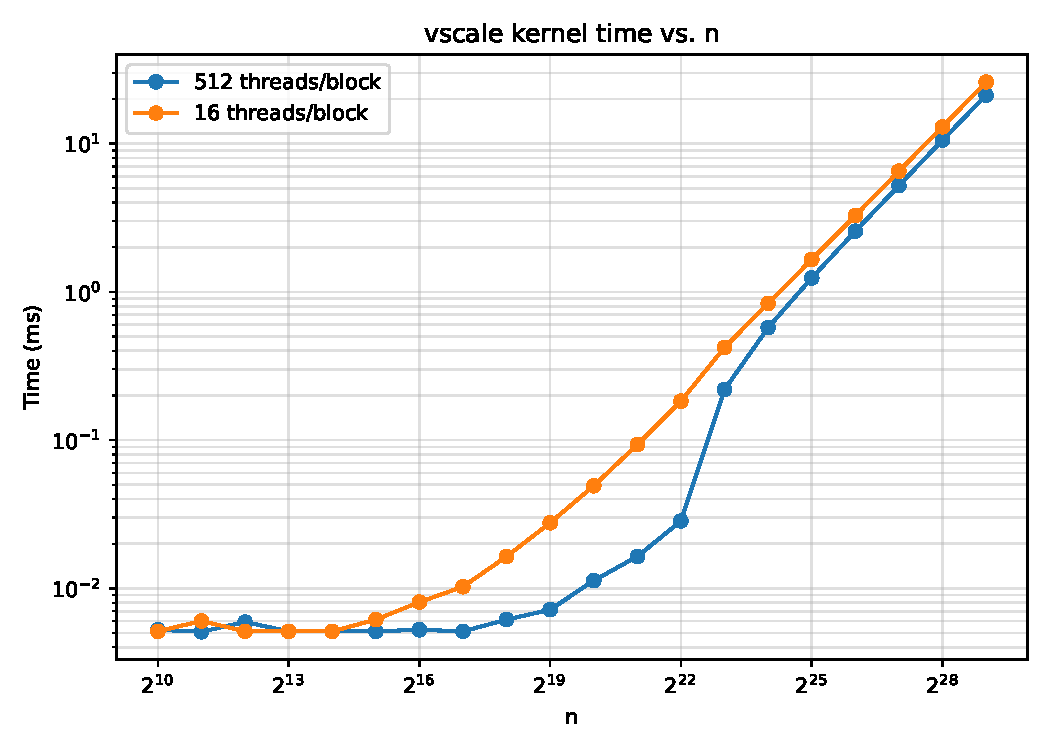
\includegraphics[width=0.7\textwidth]{task3.pdf}
  \end{center}
  \begin{itemize}
    \item \textbf{Small $n$:} both take the same time ($\approx 5\,\mu$s), since the fixed kernel start-up cost hides the tiny amount of work.
    \item \textbf{Medium $n$:} 16 threads per block is slower, since a block of 16 fills only half of a 32-thread warp, leaving half the lanes idle.
    \item \textbf{Large $n$:} the gap shrinks, since both spend most of their time reading and writing the data.
  \end{itemize}
\end{enumerate}

\end{document}
